\clearpage
\VerdierPhysicalPageAnchor{0055}%
\VerdierSemanticAnchor{ch1-1-5-4-eq4}
以上より、性質 $P(\lambda,\mu)$ は次の場合に成り立つ：

\begin{equation}
  \begin{gathered}
    \lambda\ \text{と}\ \mu\in\mathbb Z^{n-1},\\
    \lambda\ \text{と}\ \mu\in\mathbb Z e_n,\\
    \lambda\in\mathbb Z^{n-1}\ \text{かつ}\ \mu\in\mathbb Z e_n,\\
    \lambda\in\mathbb Z e_n\ \text{かつ}\ \mu\in\mathbb Z^{n-1}.
  \end{gathered}
  \tag{1.5.4.4}
\end{equation}

さらに (1.5.5) により：

\VerdierSemanticAnchor{ch1-1-5-4-eq5}
\begin{quote}
  \noindent\textup{(1.5.4.5)}\quad
  \emph{性質 $P(\mu,\nu)$、$P(\lambda+\mu,\nu)$、
  $P(\lambda,\mu+\nu)$、$P(\lambda,\mu)$ のうち三つが成り立てば、
  残る一つも成り立つ。}
\end{quote}

\VerdierSemanticAnchor{ch1-1-5-4-conclusion}
したがって性質 $P(\lambda,\mu)$ は任意の対
$\lambda,\mu\in\mathbb Z^n$ について成り立つ。これで命題 (1.5.2) の
証明が完了する。

\VerdierSemanticAnchor{ch1-1-5-5}
\noindent\textbf{図式 1.5.5.}\quad
主張 (1.5.4.5) を証明しよう。図式
$\textup{(1.5.4.1)}_{\lambda,\mu}$ を $D(\lambda,\mu)$ と書く。
(1.5.4.5) の証明は次の図式に基づく。簡単のため、遷移同型 $c,c'$ が
恒等射である場合、すなわち群 $\mathbb Z^n$ が圏 $\mathcal C,\mathcal C'$
に厳密に作用する場合について書く：

\VerdierSemanticAnchor{ch1-1-5-5-tetrahedron}
\begin{center}
  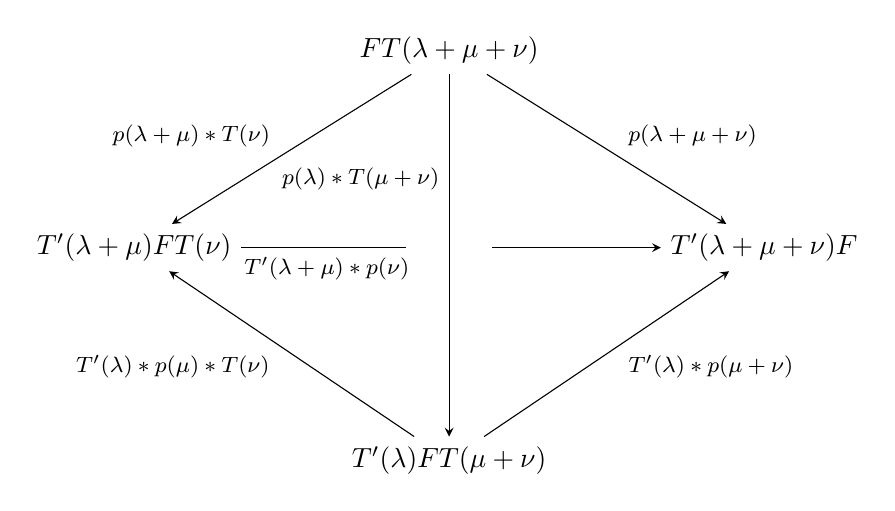
\begin{tikzpicture}[x=1cm,y=1cm,>=stealth]
    \node (a) at (0,3.2) {$FT(\lambda+\mu+\nu)$};
    \node (b) at (-4,0.7) {$T'(\lambda+\mu)FT(\nu)$};
    \node (c) at (4,0.7) {$T'(\lambda+\mu+\nu)F$};
    \node (d) at (0,-2.0) {$T'(\lambda)FT(\mu+\nu)$};
    \draw[->] (a) -- node[above left,pos=.55,font=\footnotesize]
      {$p(\lambda+\mu)*T(\nu)$} (b);
    \draw[->] (a) -- node[above right,pos=.55,font=\footnotesize]
      {$p(\lambda+\mu+\nu)$} (c);
    \draw[->] (a) -- node[left,pos=.29,font=\footnotesize]
      {$p(\lambda)*T(\mu+\nu)$} (d);
    \coordinate (bc-left) at (-0.55,0.7);
    \coordinate (bc-right) at (0.55,0.7);
    \draw (b) -- node[below,pos=.52,font=\footnotesize]
      {$T'(\lambda+\mu)*p(\nu)$} (bc-left);
    \draw[->] (bc-right) -- (c);
    \draw[->] (d) -- node[below left,pos=.55,font=\footnotesize]
      {$T'(\lambda)*p(\mu)*T(\nu)$} (b);
    \draw[->] (d) -- node[below right,pos=.55,font=\footnotesize]
      {$T'(\lambda)*p(\mu+\nu)$} (c);
  \end{tikzpicture}
\end{center}

\VerdierSemanticAnchor{ch1-1-5-5-faces}
この図式は四面体の形をしており、その四面はそれぞれ
$D(\lambda,\mu+\nu)$、$D(\lambda+\mu,\nu)$、
$D(\lambda,\mu)T(\nu)$、$T'(\lambda)D(\mu,\nu)$ である。
四つの場合を考え、余サイクル関係を用いれば (1.5.4.5) が得られる。

\VerdierSemanticAnchor{ch1-1-5-5-reduction}
一般の場合に導入すべき図式はもう少し複雑だが、恒等式 (1.2.1.3) を用いれば、
論証は上で概説したものに帰着する。(1.5.3.5) の証明には同じ図式で
\[
  \lambda=qe_1,\qquad \mu=q'e_1,\qquad \nu=q''e_1
\]
とおけばよい。
